\clearpage
\chapter{Introducción}
\label{chapter:Introduccion}
\section{Introducción}
\label{chap1:sec:introduccion}
La Microbiología es la ciencia que estudia a los microorganismos en relación a su estructura, fisiología, genética, taxonomía y aplicaciones. Estudia a los microorganismo de forma holística y en cada una de sus estructuras.

Un microorganismo es un ente biológico acelular, unicelular, pluricelular o cenocítico sin organización tisular y que requiere una metodología especial de estudio (cultivo puro)
\section{Cronología y <<Teoría de la Generación espontánea>>}
\label{chap1:sec:cronologia}
Algunos hechos notables en la historia de esta disciplina son:
\begin{itemize}[itemsep=0pt,parsep=0pt,topsep=0pt,partopsep=0pt]
	\item \textbf{Hoocke}: descubrimiento de los cuerpos fructíferos de hongos
	\item \textbf{A. van Leeuwenhoek}: descubrimiento de ciertas bacterias o “animálculos”
	\item \textbf{R. Koch}: Observación del Bacillus anthracis
	\item Microscopios y lentes de Abbe y Zeiss
	\item \textbf{Ziehl} y \textbf{Neelsen}: descripción del Mycobacterium tuberculosis
	\item \textbf{C. Gram}: tinción selectiva para microorganismos
	\item \textbf{Loeffter}: Tinción de flagelos.
\end{itemize}

\paragraph{Generación espontánea}: hasta mediados del siglo XIX, la única teoría aceptada para el origen de la vida era por generación espontánea. Los experimentos de Francesco Redi en el siglo XVII la invalidaron para seres pluricelulares. El descubrimiento del $0_2$ y de la química de los gases, junto con las controversias entre Needham y Spallanzani mantuvieron vivo el debate hasta la llegada de Pasteur, quien aboliría la teoría para el mundo microbiano.  

Los experimentos de Pasteur consistían en calentar para desinfectar un caldo de carne en un matraz. Curvó el cuello del matraz en forma de ese itálica para aislarlo del exterior, pero que siguiese entrando O2. Al no observar contaminación, probó a romper la boca del matraz, dejando expuesto el caldo de cultivo, que esta vez sí se infectó. Así, por tanto, dedujo Pasteur que la contaminación solo podía venir de microorganismo que estaban en el aire, y no se generaban espontáneamente.

Tyndall descubrió que el calor no siempre mataba a los microorganismos, no a todos. Así, observó que en cultivos a base de infusiones de heno, no todos los microorganismos eran termolábiles, algunos resistían las altas temperaturas y lo contaminaban. Fue el investigador Ferdinand Cohn quien descubrió que los microorganismos termorresistentes forma una estructura, la endospora, que sobrevivía a su forma vegetativa. Esta estructura de resistencia es muy común del género \textit{Bacillus}.
\section{Microorganismos y Ciclos biogeoquímicos. Transformación de materia. Patogenia}
\label{chap1:sec:totumrevolutum}
Los microorganismos juegan papeles bastante reseñables en la transformación de materia y patogenia. Uno de los primeros investigadores en estos campos fue Pasteur, quien describió las fermentaciones alcohólica, láctica y butírica, así como el aislamiento del primer ser anaerobio estricto, \textit{Clostridium}.

Para el estudio de microorganismo es necesaria una metodología especial, que es el cultivo puro, es decir, su aislamiento en ciertos medios para su estudio. La primera técnica fue creada por Joseph Lister (1878) por diluciones. Le siguió Emil Hansen (1886) con las diluciones seriadas. Robert Koch propuso el método de cultivo en medio sólido. En una base de agar-agar, inerte y no comestible, al añadírsele a un líquido, este se solidificaba. Creador del asa de siembra, descubrió que todos los organismos provenientes de una masa aislada en cultivo procedían del mismo individuo, que había formado una colonia.

Los primeros investigadores en relacionar a los microorganismos con los ciclos biogeoquímicos fueron Beijerinck y Winogradsky. Beijerinck, que ideó además el cultivo por enriquecimiento, descubrió que intervenían en el ciclo del nitrógeno al fijar nitrógeno molecular en el suelo, siendo los géneros \textit{Rhizobium} (en simbiosis) y \textit{Azotobacter}. Winogradsky fue el primero en observar la autotrofía en bacterias quimiolitotrofas (obtenían el carbono del $CO_2$ ambiental y la energía de reacciones químicas inorgánicas).

La idea de que algunos microorganismos podían originar enfermedades nació a partir de 1850, cuando Ignaz Semmelweis propuso que estos seres podían ser la causa de la fiebre puerperal. En 1860, Lister, en busca de prevenir estas enfermedades, lanzó la idea de la cirugía aséptica, con escaso éxito. Pero el científico que más trabajo en el campo de los microorganismos patógenos, fue Robert Koch. Asiló a los agentes del carbunco (\textit{Bacillus anthracis}) y de la tuberculosis (\textit{Mycobacterium tuberculosis}, o bacilo de Koch). Así mismo, desarrolló los postulados de Koch que permiten establecer si una enfermedad es causada o no por un microorganismo. Son:
\begin{enumerate}[itemsep=0pt,parsep=0pt,topsep=0pt,partopsep=0pt]
	\item El agente patógeno se halla en individuos enfermos, pero no en sanos
	\item Es posible aislar en medio de cultivo el patógeno en sangre del individuo enfermo
	\item Si se le inocula a un individuo aislado el microorganismo aislado, enferma.
	\item Es posible volver a aislar el patógeno en la sangre de un individuo inoculado, que es igual al del primer individuo.
\end{enumerate}
\begin{figure}[htbp]
	\centering
	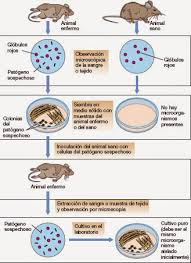
\includegraphics[trim={0 2cm 0 0},clip,width=0.8\columnwidth]{./A.imagenes/ACV-MICROBIO-PostuladosKoch}
	\caption[Postulados de Koch]{Representación de los postulados de Koch. \textit{\textbf{Extraido de}}: \protect\cite{Brock2012}}
\end{figure}

Además de las bacterias y otros microorganismos patógenos, existen otros agentes causantes de enfermedades, capaces de atravesar filtros microscópicos que las bacterias eran incapaces por su tamaño, los virus. El primero en ser descubierto fue el virus del mosaico del tabaco por Beijerinck e Ivanovsky. Así les siguieron el de la glosopeda (Loffler y Frosch), los bacteriófagos (Twort y D'Herelle). Importantes fue también la hipótesis sobre la replicación del virus del sarcoma de Rous (Temin), o el descubrimiento del VIH (Montaigner, Gallo).

En el desarrollo de la quimioterapia, una idea fundamental fue el concepto de <<bala mágica>> de Paul Erlich, que desarrolló el Salvarsán (compuesto 606) frente a la sífilis. Domayeck descubrió que el colorante Prontosil rubrum era efectivo contra estafilococos y estreptococos. Pero no fue hasta 1929 en él se creó el concepto de antibiótico con el descubrimiento de la penicilina por A. Fleming a partir de Penicilium notatum. Fueron Florey y Chain quienes consiguieron aislar en cultivos y producirla a gran escala. Para 1940, Selmen Walkman descubrió la actinomicina, la estreptomicina y la neomicina.

Un hito importante en la relación entre microorganismos y patogenia fue la creación de las vacunas  por Edward Jenner a finales del siglo XVIII. Al observar que las vaqueras en contacto con vacas con la variante bovina de la viruela eran inmunes a la cepa humana, descubrió que inoculando las costras del ganado en humanos, estos se inmunizaban. Pasteur, que utilizaba microorganismos sin poder patogénico pero sí inmunológico, creó vacunas atenuadas para la rabia o al cólera aviar. Salmon y Smith descubrieron que los microorganismos muertos por procesos físicos o químicos podían provocar inmunidad en caso de ser inoculados. Así se crearon vacunas contra la fiebre tifoidea (Widal), cólera (Haffkine) o tuberculosis, cólera, rabia y tifus (Clúa)

En el campo de la genética, algunos microorganismos o microbiólogos han tenido relación con grandes avances en esta rama. Así, el Dogma Central de la Biología Molecular de  <<1 gen: 1 enzima>> fue comprobado mediante experimentos con el moho rojo del pan, diseñados por Beadle y Tatum. La técnica de la PCR desarrollada por Kary Mullis para la clonación de genes usó enzimas de microorganismos que intervenían en la replicación del DNA.
\section{Aplicaciones de la Microbiología}
\label{chap1:sec:aplicaciones}
Los microorganismos son los seres vivos mejor conocidos dado su simplicidad estructural. Ello, junto con la facilidad de manipulación genética y su elevada tasa de crecimiento, permite usarlos para ciertos procesos con interés para los humanos en diferentes áreas, por transformación química de sustratos. Así, en la industria alimentaria pueden ser utilizados para la mejora de producción de un determinado producto, obtención de algún compuesto o en controles de calidad. En la agricultura y la ganadería, como insecticidas biológicos, cepas fijadoras de nitrógeno (abonado) o como suplemento alimentario para ganado. En el cuidado del medio natural, pueden servir para la biorremediación de suelos, reciclado de basuras y depuración de aguas, destoxificación de efluentes,… En la lucha frente a patógenos, puede ser útil la microbiología en síntesis de nuevos fármacos, tecnología de vacunas o nuevos métodos de diagnóstico.
\section{Diversidad del mundo microbiano}
\subsection{Microorganismos con estructura celular}
Los microorganismos con estructura celular, es decir, vivos, se pueden clasificar en dos grandes grupos, según presenten o no su material genético encerrado en una membrana (núcleo): procariotas (sin núcleo) y \textit{Eukarya} (con núcleo). Las procariotas a su vez se dividen en \textit{Archaea} y \textit{Bacteria}.
\subsubsection{Dominio \textit{Bacteria}}
Procariota (no presenta membrana nuclear, el material genético se presenta en el citoplasma, en una región denominada nucleoide). El material genético lo constituye, de forma general, un único cromosoma (algunos presentan mayor número) de forma circular (también se han advertido en forma lineal). Presenta también moléculas de DNA dúplex circular, con información no fundamental para el desarrollo pero que si le otorga ventajas frente a otros entes. Codifican enzimas de resistencia a antibióticos, toxinas, utilización de otros sustratos (Plásmido Tol (tolueno)).

Mayoritariamente son unicelulares, aunque a veces formen colonias o estructuras cenocíticas. La mayoría presentan pared celular, siendo de peptidoglucano (mureína). La membrana celular es muy similar a las del género \textit{Eukarya}, es decir, una estructura de bicapa lipídica enfrentando porciones hidrófobas.  En su citoplasma se hallan ribosomas de 70S y se advierta la inexistencia de orgánulos membranosos (de membrana unitaria), a excepción de los tilacoides de cianobacterias. Algunas de las funciones de los orgánulos membranosos de los eucariontes lo llevan a cabo otras estructuras, como por ejemplo la pared bacteriana, que puede realizar la función de obtención de energía de las mitocondrias. Presentan estructuras exclusivas de este dominio como son los pili o las fimbrias.

En cuanto a su morfología se pueden clasificar en cocos (esféricas), bacilos (forma de barra), espirales (forma espiral), vibrios (forma de coma). Según su motilidad, pueden ser sésiles (sin capacidad de moverse), o móviles (con capacidad de moverse, poseen una estructura particular que es el flagelo, distinto de los eucariontes). No existen procesos de reproducción sexual, se reproducen por fisión binaria. No obstante, se observan procesos de parasexualidad (intercambio de material genético): transformación, transducción y conjugación.
\subsubsection{Dominio \textit{Archaea}}
Son seres procariotas (no presenta membrana nuclear, el material genético se presenta en el citoplasma, en una región denominada nucleoide). El material genético lo constituye, de forma general, un único cromosoma de forma circular 

Este clado posee, en gran parte de sus individuos, la característica de tener pared celular, constituida en muchos casos de pseudopeptidoglucano (pseudomureína). La membrana plasmática no está formada por esteres de glicerol, sino por glicerol unido a cadenas de isoprenos (metil-1,3-butadieno) por enlaces éter. Esta característica les permite habitar lugares con condiciones ambientales límite (extremófilas). Poseen flagelos y cilios, pero de composición diferente al resto de taxones. No existen seres, en esta división taxonómica, que sean patógenos ni fotosintéticos.
\subsubsection{Dominio \textit{Eukarya}}
Este dominio se subdivide en tres grupos:
\begin{itemize}[itemsep=0pt,parsep=0pt,topsep=0pt,partopsep=0pt]
	\item \textbf{Hongos}: quimioorganotrofos heterótrofos, poseen un núcleo verdadero (eucariontes), y se alimentan por absorción. Son seres no fotosintéticos, con una pared celular de quitina y otros glucanos. Pueden reproducirse de forma asexual y sexual. Son patógenos oportunistas, sólo son invasivos en casos de inmunodepresión (\textit{Penicilium}, \textit{Aspergillus}). Se clasifican en 
	\begin{itemize}[itemsep=0pt,parsep=0pt,topsep=0pt,partopsep=0pt]
		\item \textit{\textbf{Filamentosos}}: mohos.
		\item \textit{\textbf{Unicelulares}}: levaduras.
		\item \textit{\textbf{Mucosos}}: forman esporas y son móviles. Menos desarrollados, se alimentan de bacterias.
	\end{itemize}
	\item \textbf{Algas}: eucariontes, pueden ser unicelulares de vida libre o colonial. Son fotosintéticas, con una pared celular de celulosa. Son de hábitats acuáticos.
	\item \textbf{Protozoos}: eucariontes, unicelulares. Se alimentan por ingestión. De hábitat acuático y sin pared celular. Suelen ser comensales o patógenos.
\end{itemize}
\subsection{Entidades acelulares}
\subsubsection{Virus}
Partículas infectivas, parásitos obligados, constan de una cápside proteica que encierra que encierra al material genético, que en el caso de los virus puede ser DNA o RNA, en todas la forma posibles (lineal o circular; doble o monocatenario;$\dots$). Al conjunto de cápside y material genético se le denomina nucleocápside, pudiendo estar o no recubierta de una vesícula de membrana unitaria de su anterior huésped (cubiertos o desnudos, respectivamente). Algunos virus tienen enzimas en la nucleocápside, como la lisozima o las transcriptasas, necesarias para algún proceso de su ciclo vital. Algunos virus son satélites, es decir, que necesitan de otro virus para poder infectar a una célula. Un ejemplo es el virus de la hepatitis D, que precisa infectar junto al de la hepatitis B.
\subsubsection{Viroides}
Partículas de RNA simplexo circular con estructura secundaria (especialmente puentes intracatenarios, simulando una estructura dúplex) infectivos, patógenos de plantas. Con una medida de 250 a 400 nucleótidos, se desconoce qué codifican. Fueron descubiertos por Diener en 1967. 
\subsubsection{Priones}
Moléculas patógenas formadas por proteínas, variantes conformacionales de proteínas propias, con la misma estructura primaria, pero distinta secundaria, la cual pueden transmitir a otra proteína con la conformación no patógena. Producen enfermedades como el Kuru, la encefalopatía espongiforme bovina y humana o el Corea de Huntington.
\subsection{Propuestas de clasificación}
En el momento del descubrimiento de los microorganismos, estos seres se incluyeron en los reinos ya descritos, es decir, en animales o plantas. No será hasta 1866 cuando por parte del biólogo Haeckel los clasifique, a aquellos seres sin núcleo en el reino Monera o Protista, juntando a todos los procariotas. 

En 1930, con el microscopio electrónico, Chalton establece el término procariota tras estudios de estructura celular, concepto que defendió en 1960 Murray. Para 1969, el científico Whitaker, siguiendo criterios de estructura celular, clasificó a los seres vivos en 5 reinos: \textit{Monera} (bacterias), \textit{Protoctista} (protozoos y algas), \textit{Funghi}, \textit{Plantae} y \textit{Animalia}.

En la década de 1970, al albor de la Biología Molecular, con la secuenciación de ácidos nucleicos, se pueden clasificar filogenéticamente a las especies por la similitud de estas macromoléculas. De todo el material genético celular, se estudia el RNA ribosómico (RNAr) de 16S (procariotas) ó 18S (eucariotas). Estos cronómetros moleculares se utilizan frente a otros fragmentos por su ubicuidad, su pronta aparición en la evolución, su pequeño tamaño, frente a otros genes, por la conservación de su función y de parte de la secuencia.

Propuesta por Woesse en 1977, diferenció tres dominios con un ancestro común a todos (LUCA): las bacterias por un lado, y Archaea y eucariontes por otro lado. Así, los procariotas forman un grupo bifilético frente a unas eucariotas monofiléticas.

Dentro de la clasificación de Woesse, se pueden diferenciar los siguientes subclados:
\begin{itemize}[itemsep=0pt,parsep=0pt,topsep=0pt,partopsep=0pt]
	\item \textit{\textbf{Bacteria}}: numerosos filos de los que se puede destacar \textit{Cyanobacteria}, Gram positivas, \textit{Chlamydia} (parásitos intracelulares obligados, algunos provocan ETSs), \textit{Proteobacteria} (dominio de mayoría Gram negativa, están \textit{E. colli} o \textit{Salmonella})
	\item \textit{\textbf{Archaea}}: dos filo principales: \textit{Euryarchaeota} y \textit{Crenarcheaota}. Son procariotas extremófilos.
	\item\textbf{\textit{Eukarya}}: se encuentra el reino Funghi, Plantae y Animalia.
\end{itemize}
\begin{figure}[H]
	\centering
	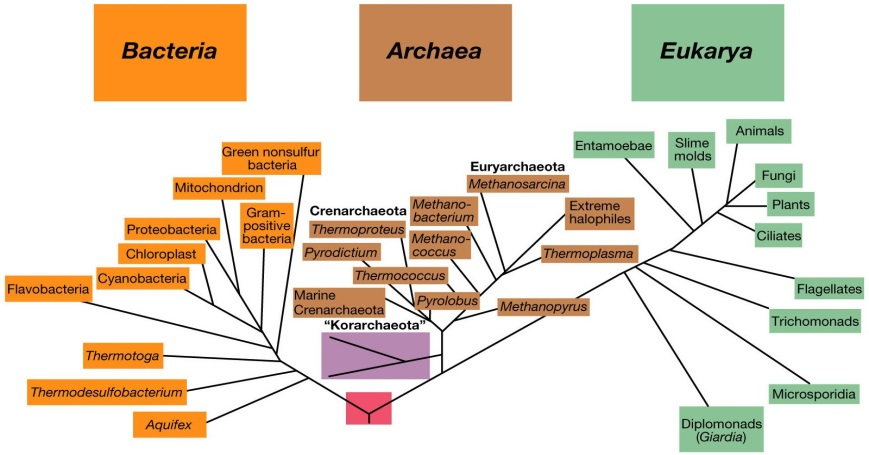
\includegraphics[width=\columnwidth]{A.imagenes/ACV-MICROBIO-PropuestaClasificacion}
	\caption[Propuesta de clasificación de Microorganismos]{Propuesta de clasificación de Microorganismos. Todas descenderían de un mismo replicador que por diversas mutaciones, daría lugar al conjunto de la vida. \textit{\textbf{Extraído de}}: \cite{Prescott2011}}
\end{figure}
